% NOTES:
%    - Show how planning ties in with traversal, explain how we assume optimize-then-execute paradigm so plan is fixed
%    - Fix link queue image, arrow is the wrong way
% while traversal isn't.

\begin{frame}{Query Optimization for Link Traversal}
    \begin{columns}[T] % T aligns columns at the top
        % Left column: Image
        \begin{column}{0.6\textwidth} % Adjust width as needed
            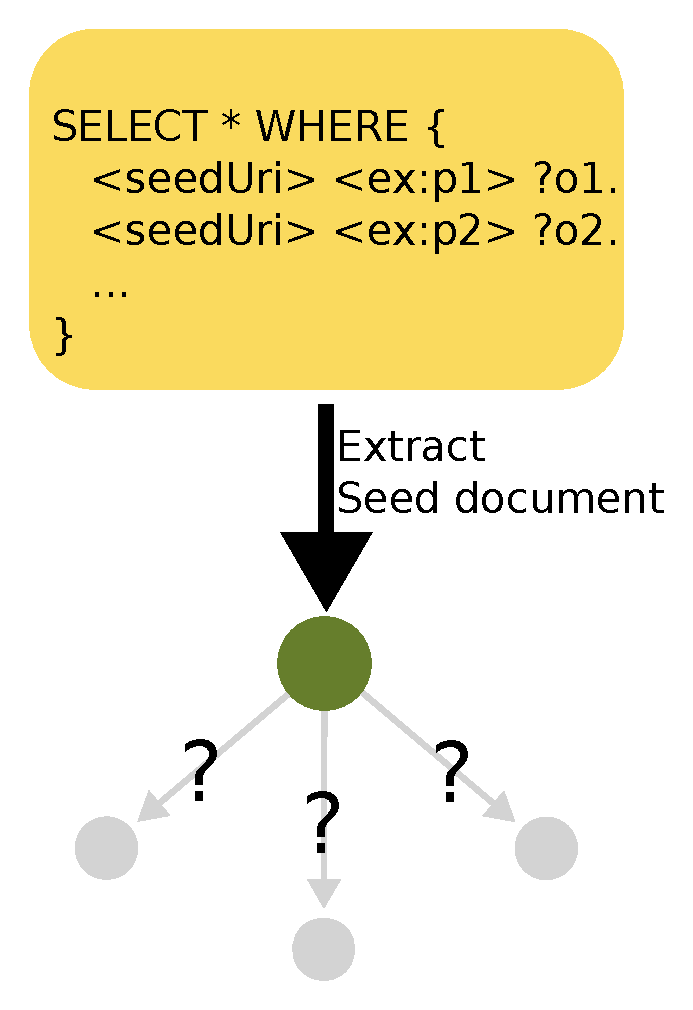
\includegraphics[width=.60\linewidth]{images/hardToOptimizeLTQP.pdf} % replace with your image file
        \end{column}

        % Right column: Text
        \begin{column}{0.4\textwidth}
            The query (partly) determines:
            \begin{itemize}
                \item The queried data
                \item The topology of the queried data
                \item The query-relevant documents
            \end{itemize}
            Result: limited prior knowledge for query optimization
        \end{column}
    \end{columns}
\end{frame}

% \begin{frame}{Query Optimization for Link Traversal: Traditional Query Planning}
%     \begin{columns}[T] % T aligns columns at the top
%         % Left column: Image
%         \begin{column}{0.6\textwidth} % Adjust width as needed
%             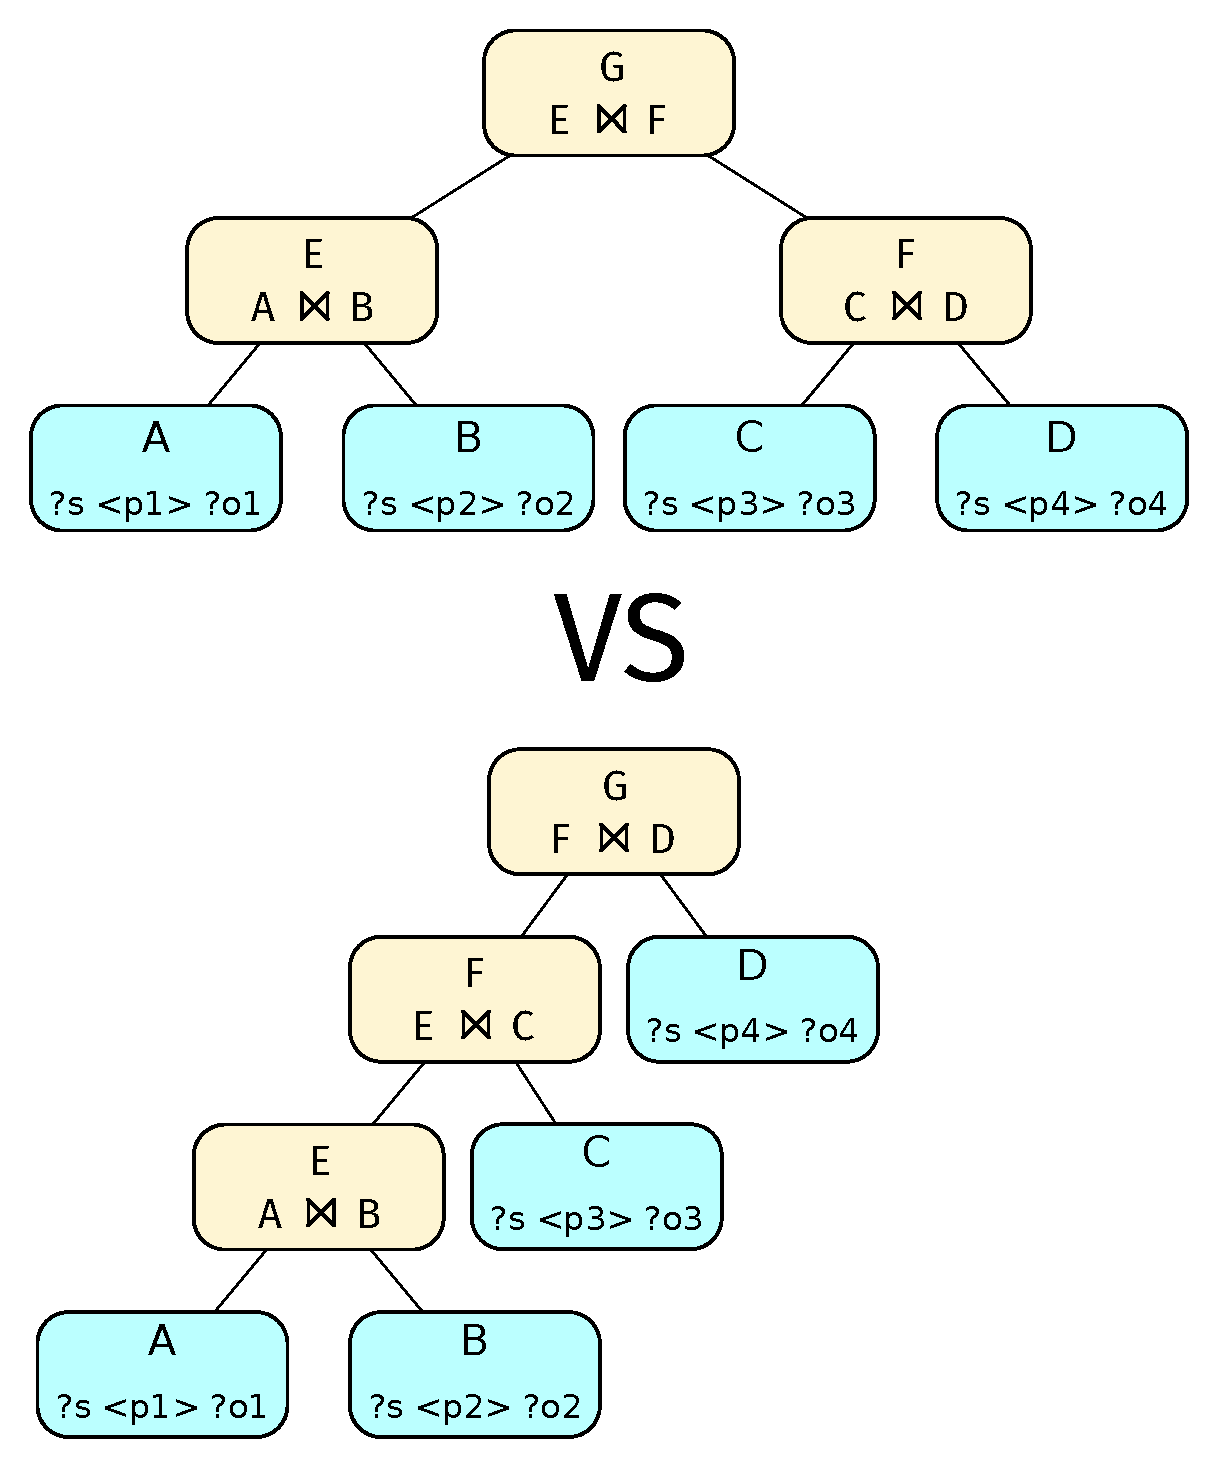
\includegraphics[width=.75\linewidth]{images/query-planning.pdf} % replace with your image file
%         \end{column}

%         % Right column: Text
%         \begin{column}{0.4\textwidth}
%             \begin{itemize}
%                 \item Query optimization for link traversal involves traditional (zero knowledge) query planning
%             \end{itemize}
%         \end{column}
%     \end{columns}
% \end{frame}

\begin{frame}{Query Optimization for Link Traversal: Traversal optimization}
    \begin{columns}[T] % T aligns columns at the top
        % Left column: Image
        \begin{column}{0.55\textwidth} % Adjust width as needed
            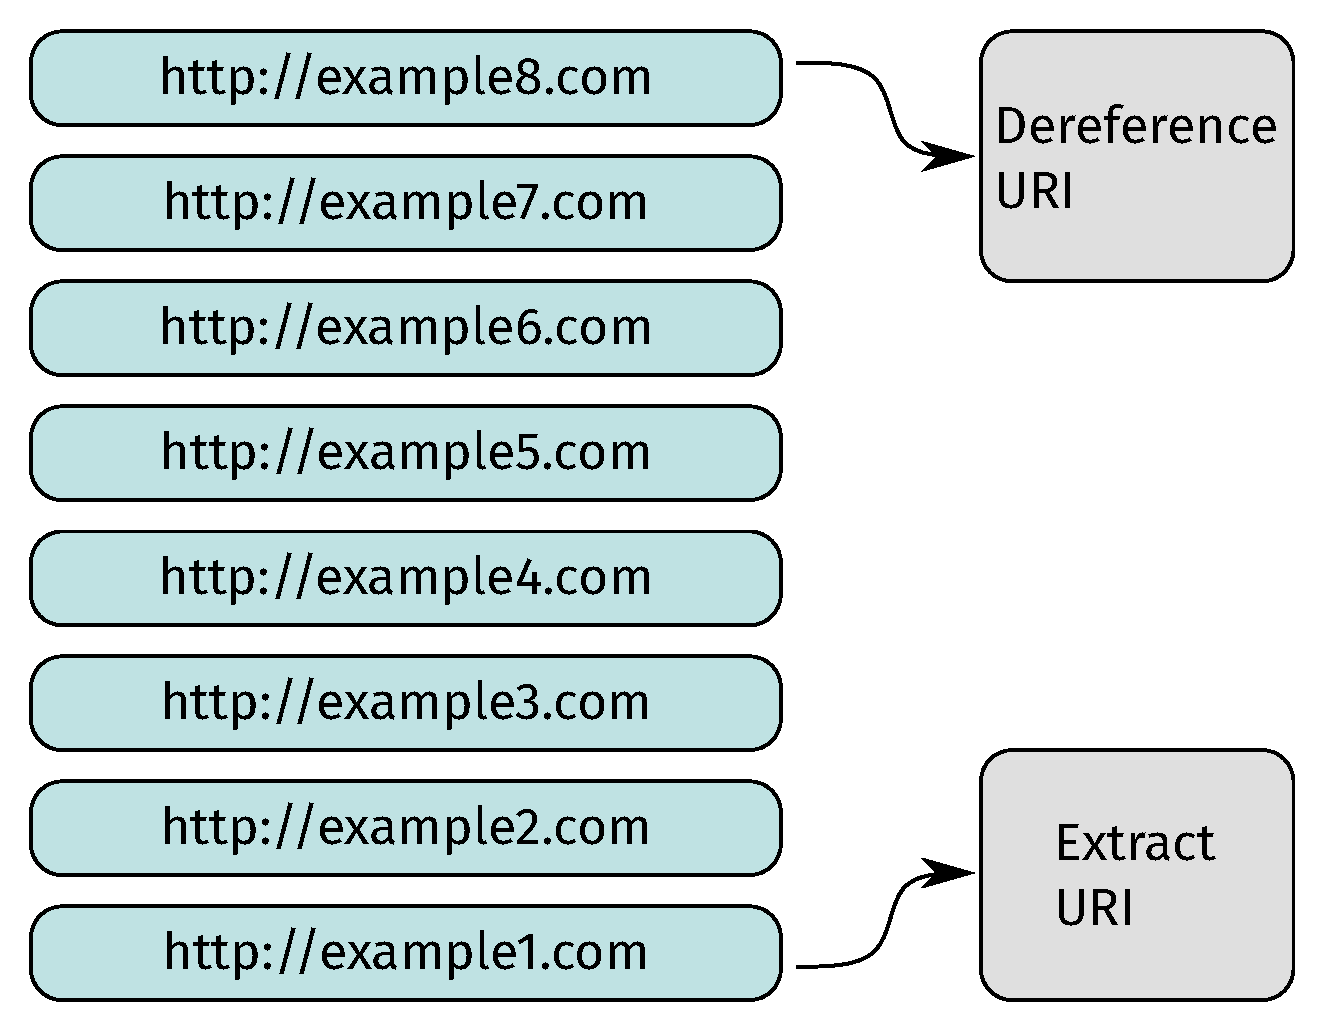
\includegraphics[width=.80\linewidth]{images/link-queue.pdf} % replace with your image file
        \end{column}

        % Right column: Text
        \begin{column}{0.4\textwidth}
            \begin{itemize}
                \item URIs are put into a link queue
                \item Link traversal uses a FiFo queue by default
            \end{itemize}
        \end{column}
    \end{columns}
\end{frame}


\begin{frame}{Query Optimization for Link Traversal: Traversal optimization}
    \begin{columns}[T] % T aligns columns at the top
        % Left column: Image
        \begin{column}{0.6\textwidth} % Adjust width as needed
            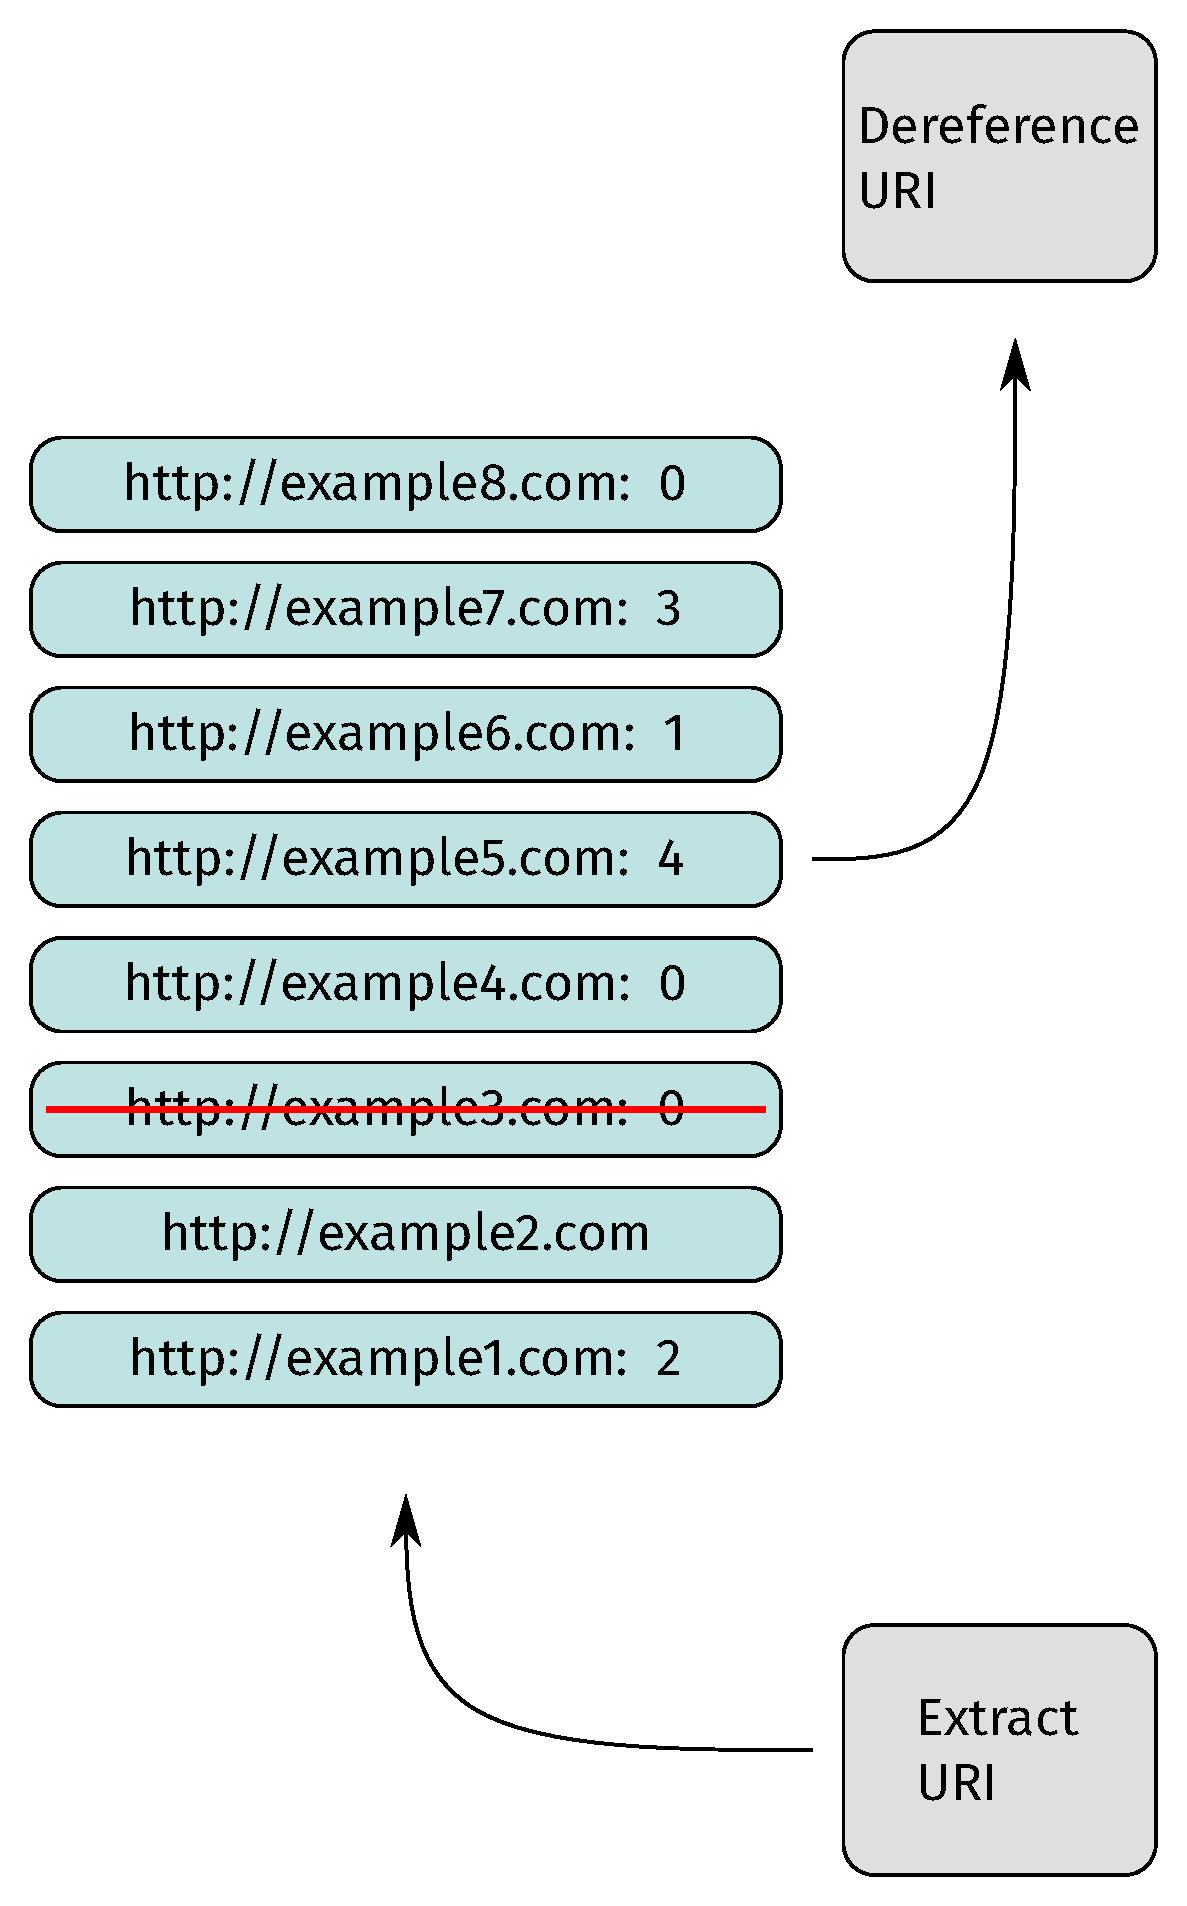
\includegraphics[width=.80\linewidth]{images/link-queue-optimized.pdf} % replace with your image file
        \end{column}

        % Right column: Text
        \begin{column}{0.4\textwidth}
            Optimizations:
            \begin{itemize}
                \item Prioritize query-relevant URIs
                \item Prune irrelevant URIs
                \item Pruning can lead to missing results without prior knowledge
            \end{itemize}
        \end{column}
    \end{columns}
\end{frame}

